\begin{figure}[h!]
	\centering
	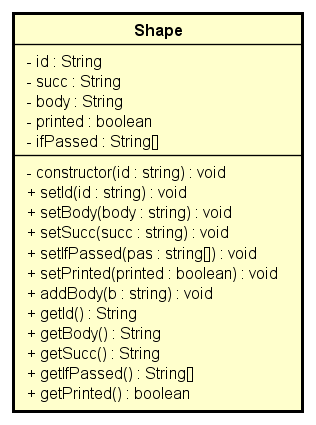
\includegraphics[scale=0.8]{res/sections/SpecificaFrontEnd/Services/Disegnetti/shape.png}
	\caption{Diagramma della classe Shape}
\end{figure}

\begin{itemize}
	\item \textbf{Descrizione:}\\
	
	\item \textbf{Utilizzo:}\\
	
	\item \textbf{Metodi:}
		\begin{itemize}
			\item \emph{-id: string}\\
    		
    		\item \emph{-succ: string}\\
    		
    		\item \emph{-body: string}\\
    		
    		\item \emph{-printed: boolean}\\
    		
    		\item \emph{-ifPassed: String[]}\\
    		
		\end{itemize}
	\item \textbf{Metodi:}
		\begin{itemize}
			\item \emph{-constructor(id: string)}\\
    		\\
    		\textbf{Parametri:}
    		\begin{itemize}
    			\item \emph{id: string}\\
    			
    		\end{itemize}
    		\item \emph{+setId(id: string)}\\
    		\\
    		\textbf{Parametri:}
    		\begin{itemize}
    			\item \emph{id: string}\\
    			
    		\end{itemize}
    		\item \emph{+setBody(body: string)}\\
    		\\
    		\textbf{Parametri:}
    		\begin{itemize}
    			\item \emph{body: string}\\
    			
    		\end{itemize}
    		\item \emph{+setSucc(succ: string)}\\
    		\\
    		\textbf{Parametri:}
    		\begin{itemize}
    			\item \emph{succ: string}\\
    			
    		\end{itemize}
    		\item \emph{+setIfPassed(pas: string[])}\\
    		\\
    		\textbf{Parametri:}
    		\begin{itemize}
    			\item \emph{pas: string[]}\\
    			
    		\end{itemize}
    		\item \emph{+setPrinted(printed: boolean)}\\
    		\\
    		\textbf{Parametri:}
    		\begin{itemize}
    			\item \emph{printed: boolean}\\
    			
    		\end{itemize}
    		\item \emph{+addBody(b: string)}\\
    		\\
    		\textbf{Parametri:}
    		\begin{itemize}
    			\item \emph{b: string}\\
    			
    		\end{itemize}
    		\item \emph{+getId()}\\
    		
    		\item \emph{+getBody()}\\
    		
    		\item \emph{+getSucc()}\\
    		
    		\item \emph{+getIfPassed()}\\
    		
    		\item \emph{+getPrinted()}\\
    		
    	\end{itemize}
\end{itemize}